% Possible types of documents/theses
%   doctype=bachelorsthesis
%   doctype=mastersthesis
%   doctype=idp
%   doctype=phdthesis
%   doctype=studienarbeit
%   doctype=diplomarbeit
%
% Document language
%   without 'lang' attribute: English
%   lang=ngerman:             German (new orthography)
%
% Binding correction
%   BCOR=<Längenangabe>
%   Additional margin, which is invisible due to binding the book
%   The usual binding by the Fachschaft has a thickness of 1,5 cm 
%
% biblatex (citations)
%   This requires 'biber' to be used instead of 'bibtex', please
%   adapt your editor's settings accordingly!
\documentclass[doctype=mastersthesis,BCOR=15mm,biblatex]{ldvbook}%lang=ngerman


\usepackage{pgfplots}
\usepackage{tikz}
\usetikzlibrary{calc}
\usetikzlibrary{matrix}




% Look for citation sources in the database "diplomarbeit.bib"
\addbibresource{thesis.bib}


%operator declarations
\DeclareMathOperator{\rank}{rank}
\DeclareMathOperator{\triu}{triu}
\DeclareMathOperator{\tril}{tril}

\begin{document}

% Bibliographic information about the thesis, please change accordingly!
\title{Titel of the thesis}
\author{Stephan Nüßlein}
\license{CC-BY}
\supervisor{Matthias Kissel}


\maketitle[frontcover=Design1]


\chapter*{Abstract}

A summary of the research question and the important findings.
Maximum 1(!) page, contains spoilers.


\tableofcontents



% Please compile this example document including the bibliography
% database. Check the resulting document and the references for 
% correct appearance (especially the German Umlaute).
% Thus you ensure that LaTeX is detecting the character encoding
% correctly and your build chain is working.
% If it does not, please tell your supervisor.






\chapter{Introduction} 3p
Motivation Why

What others are dooing

What has been done here


Description structure


\chapter{Literature Review}
\section{Neuronal Nets}
Properties of dense matrices
Approxiamtions of dense Layer matricies
Other approaces (Low Rank+ Sparse... etc..)

\section{Matrix structures}
\subsection{Matrix structures}
In the following certain matrix structures are presented.
These have in common that the rank of sub-matrices are important.
In Semiseperable matrices the rank of the lower and upper triangular part are important.
Hierarchical and sequentially semiseparable matrices are concerned with the rank of subblocks of matrices.  

\subsection{Semiseperable matricies}
Semiseperable Matrices are not consistently defined in the literature. The following is uses the definitions described in \cite{vandebril_bibliography_2005,}.
An important differentiation are generator representable semiseparable matrices and semiseparable matries.
\paragraph{Generator Representable Semiseparable Matrix}
A matrix $S$ is a generator representable semiseparable matrix if the lower and upper triangular parts of $S$ are taken from rank 1 matrices.
This can be expressed as 
\begin{align}
	\triu(S) &= \triu(pq^\top)\\
	\tril(S) &= \tril(uv^\top)
\end{align}
Where $\triu$ is the upper triangular matrix and $\tril$ is the lower triangular matrix. The vectors $p,q,u$ and $v$ are called the generators.
It is important to note here that the diagonal of $S$ is both included in the lower and upper triangular matrix.
A extension of this matrix class are the semiseparable plus diagonal matrices.  


\paragraph{Semiseparable Matrix}
In a Semiseperable matrix every subblock selected from the lower triangular part of $S$ have rank 1. The analogous statement has to be fulfilled for the upper triangular part.
This can be formalized as 
\begin{align}
	\rank(S_{i:n,1:i}) &\leq 1 & \forall_i &\in\{i,\dots,n\}\\
	\rank(S_{1:i,i:n}) &\leq 1 & \forall_i &\in\{i,\dots,n\}
\end{align}


\paragraph{Quasiseparable Matrix}
The quasiseparable matrices are similar to the Semiseperable matries. In a quasiseparable matrix every subblock selected from the strictly lower strictly upper triangular part of $S$ have rank 1. 
This can be formalized as 
\begin{align}
\rank(S_{i+1:n,1:i}) &\leq 1 & \forall_i &\in\{i,\dots,n\}\\
\rank(S_{1:i,i+1:n}) &\leq 1 & \forall_i &\in\{i,\dots,n\}
\end{align}



If the matrices are invertible the semiseperable matrices are related to tridiagobal matrices.
The inverses of a generator representable semiseparable matrix is a invertible irreducible tridiagonal matrix and vice versa. 
The inverse of a semiseparable matrix is a tridiagonal matrix and vice versa.
If a invertible quasiseparable is inverted, the inverse is again a quasiseparable matrix.

A quasiseperable Matrix is illustrated in Figure\,\ref{fig:quasiseperable}. All the marked submatrices have the property that their rank is 1.
\begin{figure}
	\centering
	

\begin{tikzpicture}
\matrix (m)[matrix of math nodes,left delimiter=(,right delimiter=)]
{
* &*&*&*&*&*\\
* &*&*&*&*&*\\
* &*&*&*&*&*\\
* &*&*&*&*&*\\
* &*&*&*&*&*\\
* &*&*&*&*&*\\
};

\def\offset{0.22mm}
\def\offdia{0.3mm}
\def\lw{0.19mm}

\draw[color=red  ,line width=\lw] ($(m-2-1.north west)+(-2*\offset,-\offdia)$)rectangle ($(m-6-1.south east)+(-\offdia,2*\offset)$);
\draw[color=blue ,line width=\lw] ($(m-3-1.north west)+(-1*\offset,-\offdia)$)rectangle ($(m-6-2.south east)+(-\offdia,1*\offset)$);
\draw[color=green,line width=\lw] ($(m-4-1.north west)+( 0*\offset,-\offdia)$)rectangle ($(m-6-3.south east)+(-\offdia,0)$);
\draw[color=red  ,line width=\lw] ($(m-5-1.north west)+( 1*\offset,-\offdia)$)rectangle ($(m-6-4.south east)+(-\offdia,-1*\offset)$);
\draw[color=blue ,line width=\lw] ($(m-6-1.north west)+( 2*\offset,-\offdia)$)rectangle ($(m-6-5.south east)+(-\offdia,-2*\offset)$);

\draw[color=red  ,line width=\lw] ($(m-1-2.north west)+(\offdia, 2*\offset)$)rectangle ($(m-1-6.south east)+( 2*\offset,\offdia)$);
\draw[color=blue ,line width=\lw] ($(m-1-3.north west)+(\offdia, 1*\offset)$)rectangle ($(m-2-6.south east)+( 1*\offset,\offdia)$);
\draw[color=green,line width=\lw] ($(m-1-4.north west)+(\offdia, 0*\offset)$)rectangle ($(m-3-6.south east)+( 0,\offdia)$);
\draw[color=red  ,line width=\lw] ($(m-1-5.north west)+(\offdia,-1*\offset)$)rectangle ($(m-4-6.south east)+(-1*\offset,\offdia)$);
\draw[color=blue ,line width=\lw] ($(m-1-6.north west)+(\offdia,-2*\offset)$)rectangle ($(m-5-6.south east)+(-2*\offset,\offdia)$);

\end{tikzpicture}

	\caption{Illustration of a semiseperable matrix}
	\label{fig:quasiseperable}
\end{figure}

These matrices classes can also be extended for higher ranks.
A matrix $S$ is a generator representable semiseparable matrix of semiseparability rank r if there exist the matrices $R_1$ and $R_2$ with $\rank(R_1)=r$ and $\rank(R_2)=r$ such that
\begin{align}
\triu(S) &= \triu(R_1)\\
\tril(S) &= \tril(R_2)
\end{align}

A similar definition for semiseparable matrices of semiseparability rank $r$ is given in \cite{vandebril_bibliography_2005}.
For this class of matrices and some slight alterations there are algorithms for the efficient calculation of different operations.

\subsection{Hirarchical Matrices}
The Hirarchical matrices are an approach to approximate Large Matrices. These were mainly introduced in \cite{grasedyck_theorie_2001,hackbusch_hierarchische_2009}.
The H-Matrices where developed for the solution of PDEs.
The computational cost of matrix operations is polynomial. Even for a quadratic complexity the computational cost prohibits the use of large matrices for certain applications.

It PDEs are solved numerically, they have to be discreticed in order to obtain an approxiamted solution.
As the diescretizaon already introduces errors, it is advantageous to drop the requirement that the matrix representation is exact, if this results in a reduction of the computational cost.
This can be done by partitioning the Matrix in segments. These blocks are represented by low Rank matrices. It the rank is smaller than the size of the matrix this representation is cheaper in terms of storage and in terms of computational cost.
For some small partitioned it might also be adeventagious to store the full blockmatrix.
To make this representation possible the size of the blockmatrices might have to be reduced.
This is done by dividing blocks that cannot be represented using a low rank representation.
To decide if a block has to be devided a admissabillity condition is introduced.
This is a way to predict the representability of a sumatrix.
For discretizations of PDEs this admissibility condition is usually based on the geometrical diameter and distance of the involved sets.
For other applications different admissibility conditions have to be derived.


\begin{figure}
	\centering
	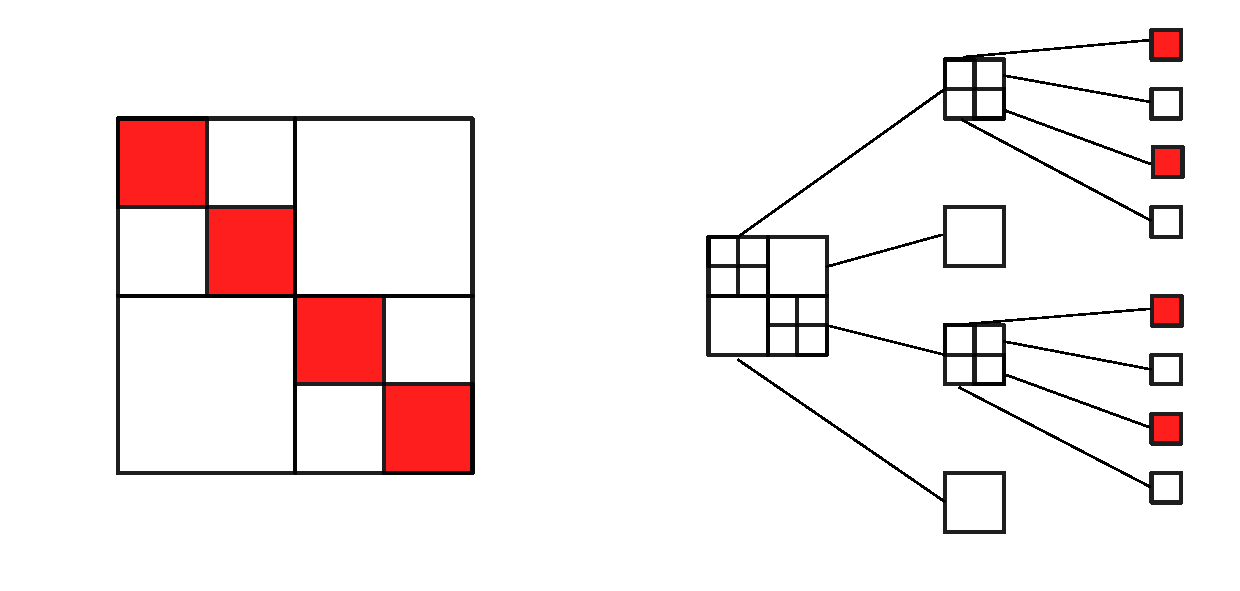
\includegraphics[width=0.7\linewidth]{diagrams/Struktur_H-matrix}
	\caption{Illustration of a $H$-Matrix and block cluster tree}
	\label{fig:strukturh-matrix}
\end{figure}


The need for efficient operations also constraints the possible sizes of the Blocks as these should be compatible.
The partition is done in a hierarchical fashion and the matrices are represented in a Block-Tree. 
If a block is not admissible, the block is divided in smaller block matrices.
If matrices are already small and still not admissible the matrices are stored directly.
Such a Tree is illustrated in Figure\,\ref*{fig:strukturh-matrix}.
In this case each non admissible block is divided in four subblocks. 
If the a block is admissible, it is stored as a low rank representations.
These are illustrated as the white rectangles.
The filled rectangles illustrate the blocks that are stored directly.
The Hierarchical matrices make it possible to compute different matrix operations efficiently.


\subsection{Sequentially semiseperable}
Sequentially semiseperable matrices were introduced in \cite{dewilde_time-varying_1998}.
As the Sequentially semiseperable maticies will be used in this thesis a introduction will be given in chapter\ref{chap:background}. 
There it will be explained form the standpoint of time varying systems.
Here the commonalities and differences to the semiseperable and hirarchical matrices are explored.

The Sequentially semiseperable matrices have the properties that submatrices have a low rank.
This is similar to semiseperable matrices. 
Unlike the semiseperable matrices this is not true for all matrices taken form the lower and upper triangular part.
The sequentially semiseperable matrices are divided into blocks.
Matrices taken form the strict lower and strict upper triangular blockmatrix have the condition that their rank is low.
This is illustrated in Figure\,\ref{fig:sequentiallysep}.

\begin{figure}
	\centering
	

\begin{tikzpicture}
\matrix (m)[matrix of math nodes,left delimiter=(,right delimiter=)]
{
* &*&*&*&*&*\\
* &*&*&*&*&*\\
* &*&*&*&*&*\\
* &*&*&*&*&*\\
* &*&*&*&*&*\\
* &*&*&*&*&*\\
};

\def\offset{0.27mm}
\def\offdia{0.2mm}
\def\lw{0.19mm}
\def\lwblk{0.3mm}

\draw[color=black ,line width=\lwblk,densely dotted] (m-1-1.north west)rectangle (m-6-2.south east);
\draw[color=black ,line width=\lwblk,densely dotted] (m-1-3.north west)rectangle (m-6-4.south east);
\draw[color=black ,line width=\lwblk,densely dotted] (m-1-5.north west)rectangle (m-6-6.south east);

\draw[color=black ,line width=\lwblk,densely dotted] (m-3-1.north west)rectangle (m-4-6.south east);

%\draw[color=red  ,line width=\lw] ($(m-2-1.north west)+(-2*\offset,-\offdia)$)rectangle ($(m-6-1.south east)+(-\offdia,2*\offset)$);
\draw[color=blue ,line width=\lw] ($(m-3-1.north west)+(-1*\offset,-\offdia)$)rectangle ($(m-6-2.south east)+(-\offdia,1*\offset)$);
%\draw[color=green,line width=\lw] ($(m-4-1.north west)+( 0*\offset,-\offdia)$)rectangle ($(m-6-3.south east)+(-\offdia,0)$);
\draw[color=red  ,line width=\lw] ($(m-5-1.north west)+( 1*\offset,-\offdia)$)rectangle ($(m-6-4.south east)+(-\offdia,-1*\offset)$);
%\draw[color=blue ,line width=\lw] ($(m-6-1.north west)+( 2*\offset,-\offdia)$)rectangle ($(m-6-5.south east)+(-\offdia,-2*\offset)$);

%\draw[color=red  ,line width=\lw] ($(m-1-2.north west)+(\offdia, 2*\offset)$)rectangle ($(m-1-6.south east)+( 2*\offset,\offdia)$);
\draw[color=blue ,line width=\lw] ($(m-1-3.north west)+(\offdia, 1*\offset)$)rectangle ($(m-2-6.south east)+( 1*\offset,\offdia)$);
%\draw[color=green,line width=\lw] ($(m-1-4.north west)+(\offdia, 0*\offset)$)rectangle ($(m-3-6.south east)+( 0,\offdia)$);
\draw[color=red  ,line width=\lw] ($(m-1-5.north west)+(\offdia,-1*\offset)$)rectangle ($(m-4-6.south east)+(-1*\offset,\offdia)$);
%\draw[color=blue ,line width=\lw] ($(m-1-6.north west)+(\offdia,-2*\offset)$)rectangle ($(m-5-6.south east)+(-2*\offset,\offdia)$);

\end{tikzpicture}

	\caption{Illustration of a sequentially semiseperable matrix. The thick dotted lines mark the segemntation of the matrix. The thin lines represent submatrices with low rank.}
	\label{fig:sequentiallysep}
\end{figure}

This segmentation in blocks makes similar to the Hirarchical Matrices that also have a segmentation.
Unlike semiseperable matrices the Sequentially semiseperable matrices do not have to be quadratic. 

\chapter{Background/Introduction}\label{chap:background}

Sequentially Semiseperable Matrices can be considered as descriptions of time varying systems.

Details on SSS systems
Hankel Operator, Reachability, Observability
Minimality
SSS as matrix factorization


\chapter{Methods} 15p

\chapter{Experiment Setups}
4pages

\chapter{Experiments}
10pages
Test it on different structures

\chapter{Discussion}
4-5 4pages

\chapter{Conclusion}
1-2 pages







% Puts out the list of references
\printbibliography{}

\end{document}
